%!TEX program = xelatex
\documentclass[UTF8,zihao=5]{ctexart} %ctex包的article


\usepackage[hidelinks]{hyperref}%超链接,自动加到目录里面



\title{{\bfseries\rmfamily\Huge{高等流体力学\hspace{1em}\\第3次作业}}}
\author{周涵宇 2022310984}
\date{}

\usepackage[a4paper]{geometry}
\geometry{left=0.75in,right=0.75in,top=1in,bottom=1in}%纸张大小和页边距

\usepackage[
UseMSWordMultipleLineSpacing,
MSWordLineSpacingMultiple=1.5
]{zhlineskip}%office风格的行间距

\usepackage{fontspec}
\setmainfont{Times New Roman}
\setsansfont{Source Sans Pro}
\setmonofont{Latin Modern Mono}
\setCJKmainfont{SimSun}[AutoFakeBold=true]
% \setCJKmainfont{仿宋}[AutoFakeBold=true]
\setCJKsansfont{黑体}[AutoFakeBold=true]
\setCJKmonofont{DengXian}[AutoFakeBold=true]

\setCJKfamilyfont{kaiti}{楷体}
\newfontfamily\CM{Cambria Math}


% \usepackage{indentfirst} %不工作 怎样调整ctex的段首缩进大小呢

\usepackage{fancyhdr}
\pagestyle{fancy}
\lhead{
    \CJKfamily{kaiti}{
        高等流体力学作业\hspace{6em}
        班级\ \ 航博221\hspace{6em}
        学号\ \ 2022310984\hspace{6em}
        姓名\ \ 周涵宇
        }
}
\chead{}
\rhead{}
\lfoot{}
\cfoot{\thepage}
\rfoot{}
\renewcommand{\headrulewidth}{0.5pt} %改为0pt即可去掉页眉下面的横线
\renewcommand{\footrulewidth}{0pt} %改为0pt即可去掉页脚上面的横线
\setcounter{page}{1}


% \usepackage{bm}

\usepackage{amsmath,amsfonts}
\usepackage{array}
\usepackage{enumitem}
\usepackage{unicode-math}

% \usepackage{titlesec} % it subverts the ctex titles
\usepackage{titletoc}


% titles in toc:
\titlecontents{section}
              [2cm]
              {\sffamily\zihao{5}\mdseries}%
              {\contentslabel{3em}}%
              {}%
              {\titlerule*[0.5pc]{-}\contentspage\hspace*{1cm}}

\titlecontents{subsection}
              [3cm]
              {\rmfamily\mdseries\zihao{5}}%
              {\contentslabel{3em}}%
              {}%
              {\titlerule*[0.5pc]{-}\contentspage\hspace*{1cm}}

\titlecontents{subsubsection}
              [4cm]
              {\rmfamily\mdseries\zihao{5}}%
              {\contentslabel{3em}}%
              {}%
              {\titlerule*[0.5pc]{-}\contentspage\hspace*{1cm}}
\renewcommand*\contentsname{\hfill \sffamily\mdseries 目录 \hfill}

\ctexset{
    section={   
        % name={前面,后面},
        number={\arabic{section}.},
        format=\sffamily\raggedright\zihao{4}\mdseries,
        indent= {0em},
        aftername = \hspace{0.5em},
        beforeskip=1ex,
        afterskip=1ex
    },
    subsection={   
        % name={另一个前面,另一个后面},
        number={\arabic{section}.\arabic{subsection}.}, %如果只用一个数字而非1.1
        format=\rmfamily\raggedright\mdseries\zihao{5},%正体字体,不加粗,main字体,五号字
        indent = {2em}, %缩进
        aftername = \hspace{0.5em},
        beforeskip=1ex,
        afterskip=1ex
    },
    subsubsection={   
        % name={另一个前面,另一个后面},
        number={\arabic{section}.\arabic{subsection}.\arabic{subsubsection}.}, %默认的 1.1.1
        format=\rmfamily\raggedright\mdseries\zihao{5},%无衬线字体,加粗,sans字体,五号字
        indent = {2em}, %缩进
        aftername = \hspace{0.5em},  %名字和标题间插入字符(此处是空白)
        beforeskip=1ex, %空行
        afterskip=1ex
    }
}

\usepackage{float}
\usepackage{graphicx}
\usepackage{multirow}
\usepackage{multicol}
\usepackage{caption}
\usepackage{subcaption}


%part、section、subsection、subsubsection、paragraph、subparagraph
\newcommand{\bm}[1]{{\mathbf{#1}}}
\newcommand{\trans}[0]{^\mathrm{T}}
\newcommand{\tran}[1]{#1^\mathrm{T}}
\newcommand{\hermi}[0]{^\mathrm{H}}
\newcommand{\conj}[1]{\overline{#1}}
\newcommand*{\av}[1]{\left\langle{#1}\right\rangle}
\newcommand*{\avld}[1]{\frac{\overline{D}#1}{Dt}}
\newcommand*{\pd}[2]{\frac{\partial #1}{\partial #2}}
\newcommand*{\pdcd}[3]{\frac{\partial^2 #1}{\partial #2 \partial #3}}
\newcommand*{\inc}[0]{{\Delta}}

\newcommand*{\uu}[0]{\bm{u}}
\newcommand*{\vv}[0]{\bm{v}}
\newcommand*{\g}[0]{\bm{g}}
\newcommand*{\nb}[0]{{\nabla}}



\begin{document}

\maketitle
\thispagestyle{fancy}


% \begin{center}
%     \rmfamily
%     \tableofcontents\setcounter{page}{0}
% \end{center}
% \thispagestyle{empty} % 目录
% \newpage %换页

\section{超声速点声源}

% 小扰动扰流问题的基本方程为:
% $$
% \frac{M^2}{U^2}\pd{^2\varphi}{t^2}
% +
% 2\frac{M^2}{U}\pd{^2\varphi}{t\partial x}
% +
% B^2\pd{^2\varphi}{x^2}
% -\pd{^2\varphi}{y^2}-\pd{^2\varphi}{z^2}
% = \delta(x)\delta(y)\delta(z)m(t)
% $$

$B=\sqrt{M^2-1}$,$M$是来流马赫数。

静止介质中超声速点源的基本解为:
$$
    \varphi = -\frac{1}{4\pi r_B}\left[
        f\left(t-\frac{D_1}{a_0}\right)
        +
        f\left(t-\frac{D_2}{a_0}\right)
        \right]
$$
其中振幅半径
$$
    r_B=\sqrt{
        (x-x_1)^2
        -B^2\left[
            (y-y_1)^2
            +(z-z_1)^2
            \right]
    }
$$
相位半径
$$
    D_1=\frac{M(x-x_1)-r_B}{B^2},\ \
    D_2=\frac{M(x-x_1)+r_B}{B^2}
$$


考虑到设马赫角为$\alpha$,
则$M=\frac{1}{\sin{\alpha}},\ B=\cot{\alpha}$,
因而有$\frac{M}{B}=\frac{1}{\cos{\alpha}},\ \frac{1}{B}=\tan{\alpha}$



设,在静止介质的坐标系中,当前声源在$O$,在$Q$
点观察。

出于绕$x$轴对称性,
下文中不妨设$z=z_1$,则可见,当$|y-y_1|<\tan{\alpha}(x-x_1)$且$x-x_1>0$,
才能使得振幅半径有意义且相位半径大于0,此时是有意义的解。这个坐标范围的
界限就是半顶角为$\alpha$的马赫锥,图中记为$OM$。

$Q$仅在马赫锥之内有意义。

考虑某个$P_i$在$x$轴上,
其是某个时间之前的声源,且在这里发出的扰动在静止的介质中,
一方面恰好达到Q处,另一方面这个传播时间之后声源到达当前的$O$。
体现在图形上,就是选$x$轴上1点$P_i$,使得其到马赫锥$OM$的距离
刚好等于$P_iQ$的长度。设这个长度为$D_i$,列方程为
$$
    (MD_i-(x-x_1))^2+(y-y_1)^2=D_i^2
$$
其有两个不同的实根:
$$
    D_{1,2}=\frac{M(x-x_1)\pm\sqrt{(x-x_1)^2-(M^2-1)(y-y_1)^2}}{B^2}
$$
化简后与基本解中的$D_1,D_2$恰好相等,即为图中$P_iM_i$或者$P_iQ$的长度($i=1,2$)。
因此,图中两个圆的半径即为相位半径$D_1,D_2$。

其中,$M_1,M_2$是$P_1,P_2$到$OM$的垂足,几何上以$P_i$为圆心$M_iP_i$为半径作圆,
要求圆恰好过$Q$点。这个约束可以确定两个$P_i$的位置。

根据图中关系,
$B\frac{D_2-D_1}{2}=\frac{r_B}{B}=\overline{M_1M_m}=\frac{\overline{M_1M_2}}{2}$,
其中$M_m$是$M_1,M_2$的中点,则作$M_mS\perp Ox$交$M_1 P_1$于$S$,可知$\overline{M_1S}=r_B$是振幅半径。

\begin{figure}[H]
    \centering
    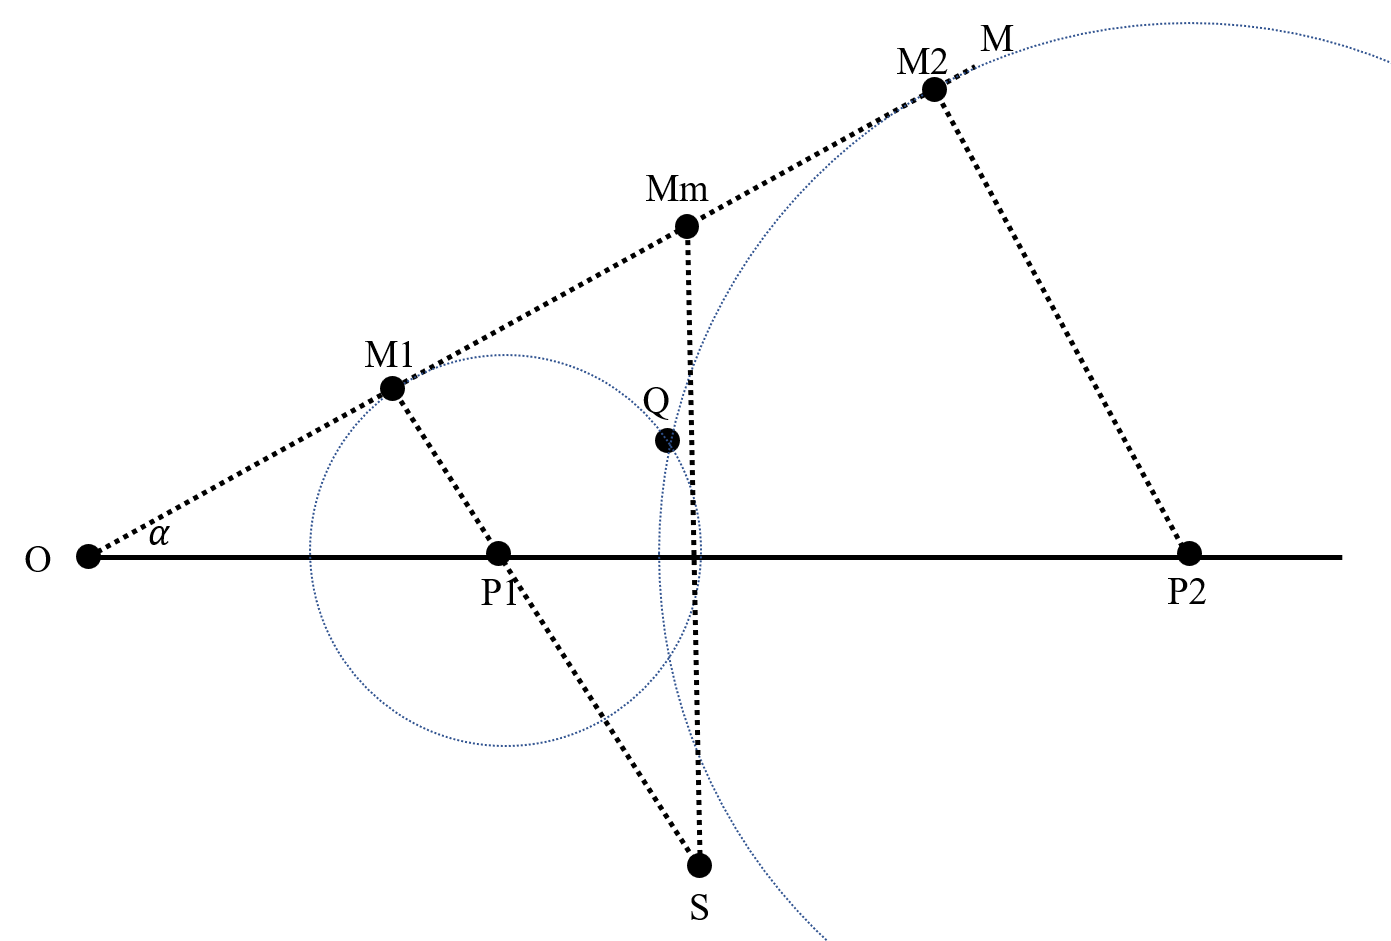
\includegraphics[width=10cm]{demo1.png}  %需调整
    \caption{振幅半径与相位半径几何结构示意}
    \label{fig:demo1}
\end{figure}

相位半径的几何意义与亚音速类似,但是亚音速情况中,相位半径只有一个有意义,而
超音速情况则有两个有意义的相位半径;这一点也体现在基本解中。

关于振幅半径,在亚声速情况下,振幅半径是声源当前位置在$PQ$的投影给出的;
而超声速情况下由于存在两个决定相位的$P$,几何上并不容易找到关系很直接的振幅半径。

另一个特点是,振幅半径在$Q$趋于马赫锥时,会趋于0,
这时的振幅趋于无穷大是奇异解,这是亚声速不存在的。

\section{群速度和相速度关系}

已知
$$
    C=\frac{\omega}{k}
$$
$$
    U=\frac{d\omega}{dk}
$$
$$
    \lambda = \frac{2\pi}{k}
$$

因此,
$$
    C=\frac{\lambda\omega}{2\pi}
$$
$$
    \frac{dC}{d\lambda}=\frac{\omega}{2\pi} + \frac{\lambda}{2\pi}\frac{d\omega}{d\lambda}
    =\frac{C}{\lambda}+\frac{\lambda}{2\pi}\frac{d\omega}{dk}\left(
    -\frac{2\pi}{\lambda^2}
    \right)
    =\left(
    C - U
    \right)
    \frac{1}{\lambda}
$$

因此:
$$
    U=C-\lambda \frac{dC}{d\lambda}
$$

\section{旗帜飘动}

将来流看作势流,记号与课本$3.4.3$保持一致,设
上下边界为无穷远,来流$x$方向,速度为$U$。有速度势的通解:

$$
    \begin{aligned}
        \varphi_1(x,z,t) & = Ux + Ae^{-kz}\exp{[ik(x-ct)]} \\
        \varphi_2(x,z,t) & = Ux + Be^{kz}\exp{[ik(x-ct)]}
    \end{aligned}
$$

设分界面为:
$$
    z=\zeta(x,t)=D\exp{[ik(x-ct)]}
$$
线化运动学(旗帜)边界条件:
$$
    \begin{aligned}
        \pd{\zeta}{t} + U\pd{\zeta}{x} & =\pd{\varphi_1}{z} \\
        \pd{\zeta}{t} + U\pd{\zeta}{x} & =\pd{\varphi_2}{z} \\
    \end{aligned}
$$
得到
$$
    \begin{aligned}
        iD(U-c)=-A=B
    \end{aligned}
$$
根据自由面动力学边界条件
$$
    \begin{aligned}
        p_1=\rho\left[-\pd{\varphi_1}{t}-U\left(\pd{\varphi_1}{x}-U\right)\right] \\
        p_2=\rho\left[-\pd{\varphi_2}{t}-U\left(\pd{\varphi_2}{x}-U\right)\right] \\
    \end{aligned}
$$
可知动力学约束为
$$
p_1-p_2=-2Dk\rho\left(
    U-c  
\right)^2
\exp{[ik(x-ct)]}
$$
其中,由于旗子微元受到张力、惯性力影响,有:
$$
p_1-p_2-\gamma\pd{^2\zeta}{x^2}=-m\pd{^2\zeta}{t^2}
$$
可知
$$
p_1-p_2=(-\gamma Dk^2 + mDk^2c^2)\exp{[ik(x-ct)]}
$$
因此有关系:
$$
-\gamma Dk^2 + mDk^2c^2 + 2Dk\rho\left(
    U-c  
\right)^2 = 0
$$
根据$\lambda=2\pi/k$整理可得
$$
-\gamma  + mc^2 + \frac{\lambda}{\pi}\rho\left(
    U-c  
\right)^2 = 0
$$
即为色散关系。




% \section{附录}
% 本文计算代码都在\href{https://github.com/harryzhou2000/HW_ACFD}{Github Repo中(点击访问)}。































% \section{SECTION 节}

% 一个

% \subsection{SUBSECTION 小节}

% 示例

% \subsubsection{SUBSUBSECTION 小节节}

% 字体字号临时调整:
% {
%    \sffamily\bfseries\zihao{3} 哈哈哈哈哈 abcde %三号 sans系列字体(一开始设置的) 加粗
%    %只对大括号范围内的后面的字有用,在标题、题注里面同样
% }
% { 
%    \CJKfamily{kaiti}\zihao{5}\itshape 哈哈哈哈哈 abcde%三号 kaiti(一开始设置的, 斜体(英文有变)
%    %只对大括号范围内的后面的字有用,在标题、题注里面同样
% }

% 一大堆一大堆一大堆一大堆一大堆一大堆一大堆一大堆一大堆一大堆
% 一大堆一大堆一大堆一大堆一大堆一大堆一大堆一大堆一大堆一大堆一大堆一大堆
% 一大堆一大堆一大堆一大堆一大堆一大堆一大堆一大堆一大堆一大堆一大堆一大堆
% 一大堆一大堆一大堆一大堆一大堆一大堆一大堆一大堆一大堆一大堆一大堆一大堆

% \begin{center}
%     居中的什么乱七八糟东西
% \end{center}


% 一个列表:
% \begin{itemize}
%     \item asef
%     \item[\%] asdf
%     \item[\#] aaa
% \end{itemize}

% 一个有序列表:
% \begin{enumerate}
%     \item asef
%     \item[\%\%] asdf
%     \item aaa
% \end{enumerate}

% 一个嵌套列表,考虑缩进:
% \begin{enumerate}[itemindent=2em] %缩进
%     \item asef \par asaf 东西东西东西东西东西东西东西东西东西东西东西东西东西东西东西东西东西东西东西东西东西东西东西东西,
%           F不是不是不是不是不是不是不是不是不是不是不是不是不是不是不是
%           \begin{itemize}[itemindent=2em]  %缩进
%               \item lalala
%               \item mamama
%           \end{itemize}
%     \item asdf
%     \item aaa
% \end{enumerate}

% \section{SECTION}

% 图片排版:

% \begin{figure}[H]
%     \begin{minipage}[c]{0.45\linewidth}  %需调整
%         \centering
%         \includegraphics[width=8cm]{RAM_O2_4660.png}  %需调整
%         \caption{第一个图}
%         \label{fig:a}
%     \end{minipage}
%     \hfill %弹性长度
%     \begin{minipage}[c]{0.45\linewidth}  %需调整
%         \centering
%         \includegraphics[width=8cm]{RAM_O4_4660.png}  %需调整
%         \caption{第二个图}
%         \label{fig:b}
%     \end{minipage}
% \end{figure}

% figure的选项为“htbp”时,会自动浮动,是“H”则和文字顺序严格一些。

% \begin{figure}[H]
%     \begin{minipage}[c]{0.45\linewidth}  %需调整
%         \centering
%         \includegraphics[width=8cm]{RAM_O2_4660.png}  %需调整
%         \label{fig:x}
%     \end{minipage}
%     \hfill %弹性长度
%     \begin{minipage}[c]{0.45\linewidth}  %需调整
%         \centering
%         \includegraphics[width=8cm]{RAM_O4_4660.png}  %需调整
%         \label{fig:y}
%     \end{minipage}
%     \caption{第三个图}
% \end{figure}

% \begin{figure}[H]
%     \centering
%     \includegraphics[width=8cm]{RAM_O4_4660.png}  %需调整
%     \label{fig:c}
%     \caption{第四个图}
% \end{figure}



% \subsection{SUBSECTION}

% 关于怎么搞表格:

% \begin{table*}[htbp]
%     \footnotesize
%     \begin{center}
%         \caption{一端力矩载荷下的结果\fontsize{0pt}{2em}} %需要学习统一设置;0代表不变?
%         \label{表2}
%         \begin{tabular}{|c|c|c|c|c|c|c|}
%             \hline
%             节点数                              & 积分方案              & 单元数                & $h=1m$                & $h=0.1m$              & $h=0.05m$             & $h=0.01m$             \\
%             \hline
%             \multirow{6}{*}{2}                  & \multirow{3}{*}{精确} & 1                     & 4.235294117647059E-08 & 1.406250000000000E-06 & 2.862823061630218E-06 & 1.439654482924097E-05 \\
%             \cline{3-7}
%                                                 &                       & 10                    & 5.975103734439814E-08 & 4.235294117646719E-05 & 1.800000000000410E-04 & 1.406249999999849E-03 \\
%             \cline{3-7}
%                                                 &                       &
%             10000                               & 5.999999915514277E-08 & 5.999996622448291E-05 & 4.799989509752562E-04 & 5.999793702477535E-02                                                 \\
%             \cline{2-7}
%                                                 & \multirow{3}{*}{减缩} & 1                     & 6.000000000000001E-08 & 5.999999999999972E-05 & 4.799999999999911E-04 & 6.000000000003492E-02 \\
%             \cline{3-7}
%                                                 &                       & 10                    & 6.000000000000071E-08 & 5.999999999999142E-05 & 4.799999999995399E-04 & 5.999999999903294E-02 \\
%             \cline{3-7}
%                                                 &                       & 10000                 & 6.000000112649221E-08 & 5.999999234537814E-05 & 4.799997501925065E-04 & 6.000037607984510E-02 \\
%             \hline

%             \multirow{6}{*}{3}                  & \multirow{3}{*}{精确} & 1                     & 6.000000000000003E-08 & 6.000000000000202E-05 & 4.800000000000831E-04 & 6.000000000056749E-02 \\
%             \cline{3-7}
%                                                 &                       & 10                    & 5.999999999999932E-08 & 6.000000000004190E-05 & 4.800000000000206E-04 & 6.000000001613761E-02 \\
%             \cline{3-7}
%                                                 &                       & 10000                 & 6.000000013769874E-08 & 5.999989495410481E-05 & 4.799942099727246E-04 & 6.000263852944890E-02 \\
%             \cline{2-7}
%                                                 & \multirow{3}{*}{减缩} & 1                     & 6.000000000000002E-08 & 6.000000000000267E-05 & 4.800000000000754E-04 & 5.999999999989982E-02 \\
%             \cline{3-7}
%                                                 &                       & 10                    & 5.999999999999899E-08 & 5.999999999987338E-05 & 4.799999999947916E-04 & 5.999999998625345E-02 \\
%             \cline{3-7}
%                                                 &                       & 10000                 & 5.999999728157785E-08 & 5.999994914321980E-05 & 4.800008377474699E-04 & 5.999472246346305E-02 \\
%             \hline

%             \multicolumn{3}{|c|}{欧拉-伯努利解} & 6.000000000000000E-08 & 6.000000000000000E-05 & 4.800000000000000E-04 & 6.000000000000000E-02                                                 \\
%             \hline
%         \end{tabular}
%     \end{center}
% \end{table*}

% 多行、多列表格的示例,基本思想是,多列的那个东西放在多列的最上面一格,下面的行要用\&来空开,也就是\&的数目
% 和普通表格一样,是列数减一;
% 多列的部分的话,就是每行内的操作,相应的\&就少了,见最后一行。

% tabular的“|c|c|c|c|c|c|c|”,意思是,竖线-居中-竖线-居中-竖线……,可以选择省略一些竖线;
% 每行之间的hline,代表贯通的横线,cline是有范围的横线。

% \subsubsection{SUBSUBSECTION}

% newcommand可以用来定义新指令,似乎基本上就是字符串替换……不太懂,总之在公式里面可以用,
% 外面也经常用。






% 公式这么写:
% \begin{equation}
%     \begin{aligned}
%         \frac{aa(x^1+x^2)}{\sqrt{x^1x^2}}
%         \nabla\times\uu
%         = & u_{j;m}\g^m\times\g^j
%         =u_{j;m}\epsilon^{mjk}\g_k
%         =u_{j,m}\epsilon^{mjk}\g_k                           \\
%         = & \frac{1}{\sqrt{g}}\left|
%         \begin{matrix}
%             \g_1       & \g_2       & \g_3       \\
%             \partial_1 & \partial_2 & \partial_3 \\
%             u_1        & u_2        & u_3
%         \end{matrix}
%         \right|
%         =\frac{\sqrt{x^1x^2}}{aa(x^1+x^2)}
%         \left|
%         \begin{matrix}
%             \g_1                        & \g_2                        & \g_3       \\
%             \partial_1                  & \partial_2                  & \partial_3 \\
%             u^1\frac{a^2(x^1+x^2)}{x^1} & u^2\frac{a^2(x^1+x^2)}{x^2} & u^3
%         \end{matrix}
%         \right|                                              \\
%         = & \frac{\sqrt{x^1x^2}}{aa(x^1+x^2)}
%         [[\g_1\,\g_2\,\g_3]]
%         diag\left(
%         u^3_{,2}-u^2_{,3}\frac{a^2(x^1+x^2)}{x^2},\,
%         u^1_{,3}\frac{a^2(x^1+x^2)}{x^1}-u^3_{,1},\, \right. \\
%           & \left.
%         u^2_{,1}\frac{a^2(x^1+x^2)}{x^2}+u^2\frac{a^2}{x^2}
%         -
%         u^1_{,2}\frac{a^2(x^1+x^2)}{x^1}-u^1\frac{a^2}{x^1}
%         \right)                                              \\
%         = & \frac{\sqrt{x^1x^2}}{aa(x^1+x^2)}
%         [[\bm{e}_1\,\bm{e}_2\,\bm{e}_3]]
%         \left[\begin{array}{ccc} a & -a & 0\\ \frac{a\,x^{2}}{\sqrt{x^{1}\,x^{2}}} & \frac{a\,x^{1}}{\sqrt{x^{1}\,x^{2}}} & 0\\ 0 & 0 & 1 \end{array}\right]              \\
%           & diag\left(
%         u^3_{,2}-u^2_{,3}\frac{a^2(x^1+x^2)}{x^2},\,
%         u^1_{,3}\frac{a^2(x^1+x^2)}{x^1}-u^3_{,1},\, \right. \\
%           & \left.
%         u^2_{,1}\frac{a^2(x^1+x^2)}{x^2}+u^2\frac{a^2}{x^2}
%         -
%         u^1_{,2}\frac{a^2(x^1+x^2)}{x^1}-u^1\frac{a^2}{x^1}
%         \right)
%     \end{aligned}
%     \label{eq:curlu}
% \end{equation}

% 如果不想带编号的公式(或者图表),用 equation* 这种环境。

% 引用,如果是引用的图表,就用表\ref{表2},图\ref{fig:a}这种,代码里是用label定义的标签来引用,
% 编号是自动生成的。公式引用一般写成:\eqref{eq:curlu}。目前这些引用自动会有超链接,反正有那个包自动
% 好像就会有……呜呜呜也不知道是怎么做到的,先这么用吧。

% \paragraph{PARA}

% 引用文献用\\cite这些,要用bibtex,暂时不做。

% \subparagraph{SUBPARA}

\end{document}